\section{Technical Background}

The technical background is all the research related to the programming part of
this bachelor project. The programming language used in this project is a
mixture of C and C++, for this part, the course of Systems Programming taught by
Prof. Carzaniga during the third semester. Then came the study of the starting
point of the project, which was divided in the logic itself and the framework
used to display the state of the simulation on the screen.

\subsection{Original project}

Before starting to write any code, it was necessary to study carefully the
original project. The starting point of chosen for this specific project was the
last commit on the \texttt{c++-port} branch. The reason for this choice is that
the project originally started fully in C (which is still the case for the
\texttt{main} branch) and C++ offers more functionalities that help for a
smoother development process.

The life-cycle of the simulation was the typical three-step process:
\begin{enumerate}
	\item \textbf{State initiation:} the state of the application is set with certain
	      starting conditions;
	\item \textbf{State update:} the state, at each frame, gets applied a set of rules that
	      govern the behaviour of the application;
	\item \textbf{Termination:} when the user stops the application, it actuates a number
	      of \texttt{cleaning} up operations.
\end{enumerate}

Just like any C/C++ project, the modules were split into different files, and
those modules where themselves split into header files and implementation files.
The header files expose the public interface which other modules can call to
execute a determine function, whereas the implementation files, as the name
suggests, offer the concrete implementation of the aforementioned functions. The
implementation files can use some static\footnote{static in the sense of C,
	i.e. visible only to the file it is declared in} functions that it can use
as auxiliary or utility functions. The header files usually expose the fields
and methods of the class (or \texttt{struct}) the module is using, if any, together
with one function for each of three steps of the life-cycle mentioned above.

\subsection{Cairo}

Cairo is a 2D graphics library with support for multiple output devices. Cairo
is designed to produce consistent output on all output media while taking
advantage of display hardware acceleration when available. The cairo API
provides operations similar to the drawing operators of PostScript and PDF.
Operations in cairo including stroking and filling cubic Bézier splines,
transforming and compositing translucent images, and antialiased text rendering.
All drawing operations can be transformed by any affine transformation (scale,
rotation, shear, etc.). Reading the
documentation\footnote{\url{https://www.cairographics.org/documentation/}}, and
more specifically the practical
tutorial\footnote{\url{https://www.cairographics.org/tutorial/}} was useful to
understand how the library works.



The Cairo drawing model relies on a three-layer model, any drawing process takes
place in three steps:

\begin{minipage}{.5\textwidth}
	\begin{enumerate}
		\item first a mask is created, which includes one or more vector
		      primitives or forms, i.e., circles, squares, TrueType fonts, Bézier
		      curves, etc;

		\item then source must be defined, which may be a color, a color
		      gradient, a bitmap or some vector graphics, and from the painted
		      parts of this source a die cut is made with the help of the above
		      defined mask;

		\item finally the result is transferred to the destination or surface,
		      which is provided by the back-end for the output.
	\end{enumerate}
\end{minipage}
\begin{minipage}{.49\textwidth}
	\centering
	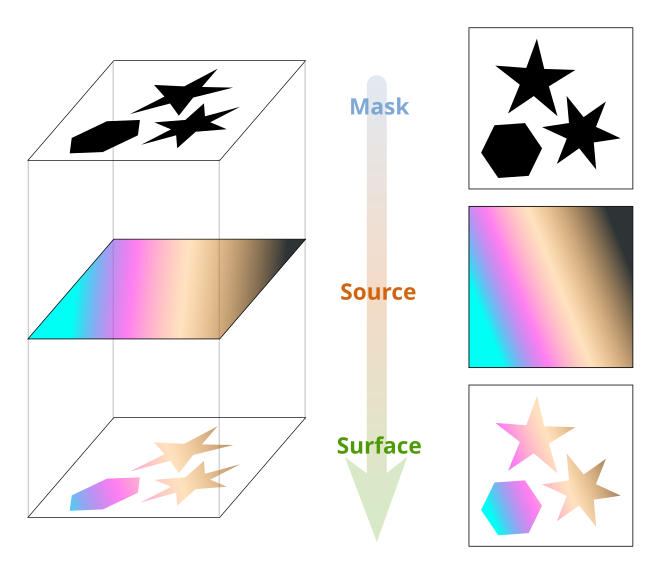
\includegraphics[width=0.8\textwidth]{cairo}
	\captionof{figure}{Cairo's drawing model}
	\label{fig:cairo}
\end{minipage}
